\documentclass[11pt, oneside]{article}   	% use "amsart" instead of "article" for AMSLaTeX format
\usepackage{geometry}                		% See geometry.pdf to learn the layout options. There are lots.
\geometry{letterpaper}                   		% ... or a4paper or a5paper or ... 
%\geometry{landscape}                		% Activate for for rotated page geometry
%\usepackage[parfill]{parskip}    		% Activate to begin paragraphs with an empty line rather than an indent
\usepackage{graphicx}				% Use pdf, png, jpg, or eps§ with pdflatex; use eps in DVI mode
								% TeX will automatically convert eps --> pdf in pdflatex		
\usepackage{amssymb}
\usepackage{pgf}
\usepackage{pdfpages}
\usepackage{tikz}
\usetikzlibrary{arrows,automata}
\usepackage[latin1]{inputenc}
\usetikzlibrary{arrows,automata}

\title{Assignment 3}
\author{James Austin}
%\date{}							% Activate to display a given date or no date

\begin{document}
\maketitle
\section{Problem 0}
\subsection{Q1,Q2, Q4}
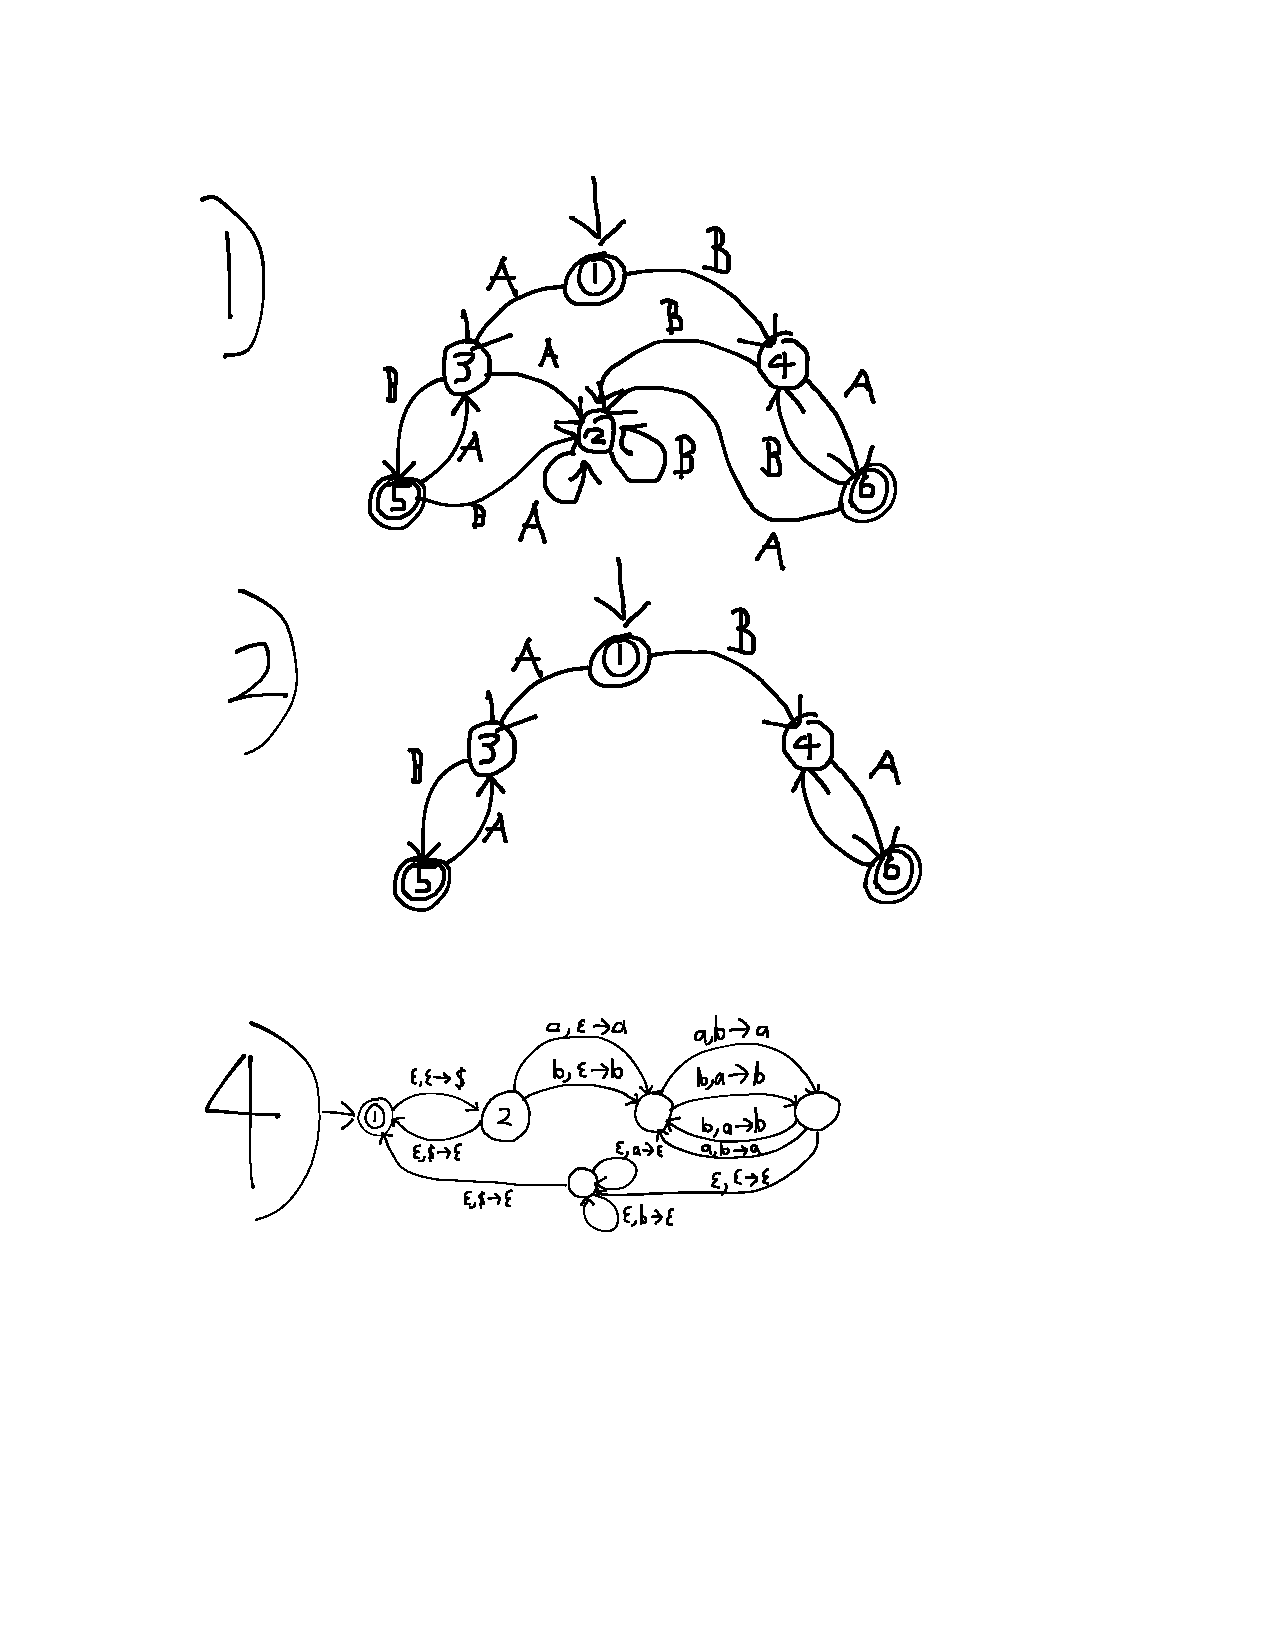
\includepdf{124.pdf}

\subsection{Q3}
$S\rightarrow \epsilon$\\
$S\rightarrow X$\\
$S\rightarrow Y$\\
$Y\rightarrow \epsilon$\\
$Y\rightarrow abY$\\
$X\rightarrow \epsilon$\\
$X\rightarrow baX$\\

\subsection{Q5}

We are aiming to prove that the string $a^nb^{2n}$ is proved by the grammar $S \rightarrow aSbb | \epsilon$ for all $n \geq 0$.

Base case: $N = 1$

The valid string for $n = 1$ is $abb$.

We can create it with $S \rightarrow aSbb \rightarrow a\epsilon bb = abb$

We can suppose that we can generate the string $a^{n+1}b^{2(n+1)}$ using the grammar. This string is equal to $aa^nb^{2n}bb$. That string can then be derived from a further expansion of the original context.

$aSbb \rightarrow ... \rightarrow a^nb^{2n}b \rightarrow aa^nb^{2n}bb$

Hence, we have proven that the string  $a^{n+1}b^{2(n+1)}$ can be derived from the original grammar. Following on from this, we can show that 

As we have shown that the base case and inductive step are correct, we have proved that every string in the language$\{a^{2n}b^n: n\leq 0 \}$ 

%\section{}
%\subsection{}



\end{document}  